\documentclass{beamer}

\usepackage[T1]{fontenc}
\usepackage{lmodern}
\usepackage{graphicx}
\usepackage[french]{babel}
\usepackage[babel=true]{microtype}
\usepackage[bookmarksopen=true]{hyperref}
\usepackage{booktabs, bookmark}

\usetheme{Dresden}

\definecolor{purple}{rgb}{0.5, 0, 1}
\setbeamercolor*{palette primary}{use=structure, fg=white, bg=purple}
\setbeamercolor*{palette secondary}{use=structure, fg=white, bg=purple}
\setbeamercolor*{palette tertiary}{use=structure, fg=white, bg=purple}
\setbeamercolor*{palette quaternary}{use=structure, fg=white, bg=purple}

\setbeamercolor*{sidebar}{fg=purple,bg=gray!15!white}

\setbeamercolor*{palette sidebar primary}{fg=purple!10!black}
\setbeamercolor*{palette sidebar secondary}{fg=white}
\setbeamercolor*{palette sidebar tertiary}{fg=purple!50!black}
\setbeamercolor*{palette sidebar quaternary}{fg=gray!10!white}

\setbeamercolor{titlelike}{parent=palette primary,bg=purple}
\setbeamercolor{frametitle}{bg=yellow!90!white, fg=purple}
\setbeamercolor{frametitle right}{bg=gray!60!white}

\title{CPU et horloge sur FPGA}
\author{
  Jean \textsc{Caspar},
  Loïc \textsc{Chevalier},
  Vladimir \textsc{Ivanov},
  Adrien \textsc{Mathieu}
}
\date{24 Janvier 2023}

\begin{document}

\frame{\titlepage}

\begin{frame}
    \frametitle{Assembleur}
    \begin{itemize}
        \item Nous avons développé un jeu d'instructions et un assembleur, en Rust
        \item Le registre $r_0$ est toujours à $0$, 15 autres registres
        \item Les instructions prennent une à deux opérandes, registres ou immédiats, et un
              registre de sortie $r_d$
        \item Opérations arithmétiques : $r_d = lhs \operatorname{op} rhs$
        \item Comparaisons $r_d = 1$ si $lhs \operatorname{cc} rhs$, $r_d = 0$ sinon
        \item Sauts : \verb|jmp|, \verb|jo|, \verb|jz|, \verb|jzo|, \verb|jnz|, \verb|jnzo|.
              $o$ désigne un saut relatif, $z$ saute si l'opérande est nulle, $nz$ si elle est non nulle
        \item RAM : \verb|load| et \verb|store|
        \item IO : \verb|recv| et \verb|send|
         
    \end{itemize}
\end{frame}

\begin{frame}
    \frametitle{Verilog}
    Le programme Verilog est séparé en plusieurs modules.
    \begin{itemize}
        \item ALU et comparateur
        \item Un pointeur d'instruction, et un module pour gérer les sauts
        \item Des registres, de la RAM et un sélecteur d'instruction
        \item Des bus et un module de gestion de l'IO
        \item Un driver qui instancie les autres modules
    \end{itemize}
\end{frame}

\begin{frame}
    \frametitle{Simulation et VM}
    \begin{itemize}
        \item VM qui simule le CPU
        \item Peut prendre en paramètre la fréquence à laquelle tourner
        \item Peut calculer le chemin critique d'un programme (ou au moins une estimation)
    \end{itemize}
\end{frame}

\begin{frame}
    \frametitle{FPGA}
    Précédemment nous avions tenté d'utiliser 12 afficheurs 7 segments pour tout afficher en même temps.
    Mais le FPGA n'a pas autant de sorties donc il aurait fallu utiliser des puces en plus pour servir
    de registres et de décodeur.
    \begin{center}
        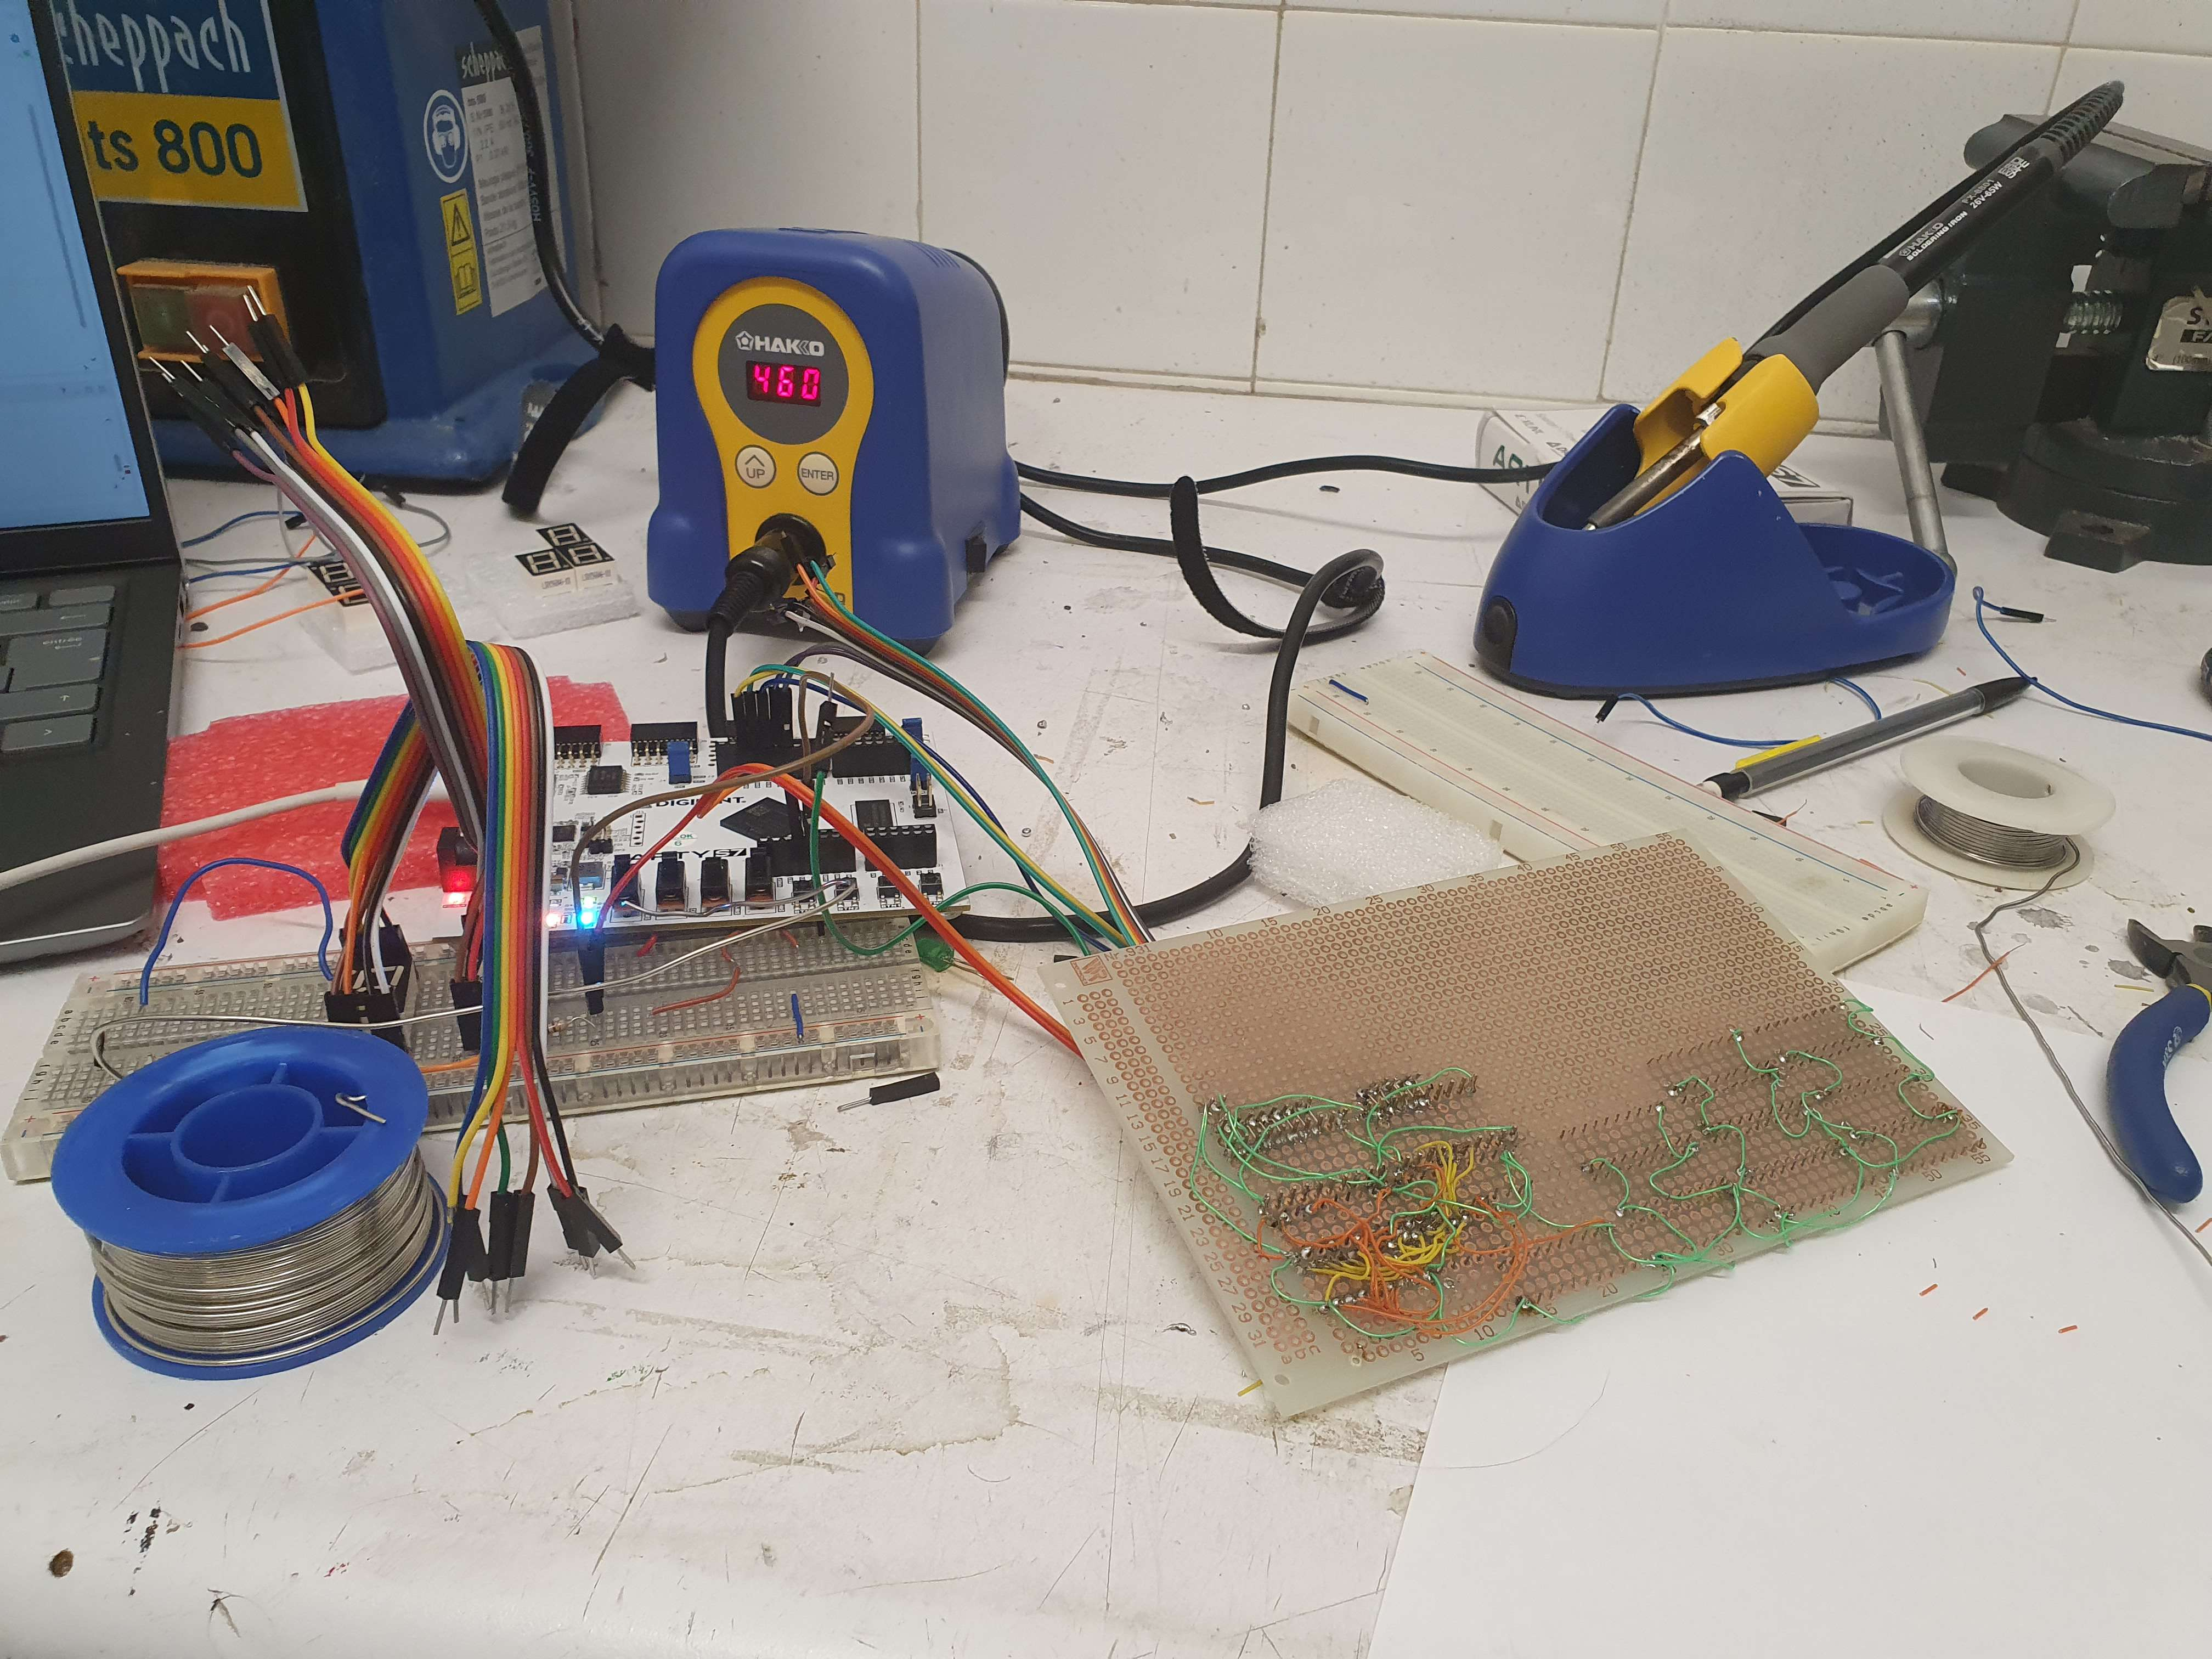
\includegraphics[scale=0.05]{pictures/Soudure global.jpg}
    \end{center}
\end{frame}

\begin{frame}
    C'est un échec :
    \begin{center}
        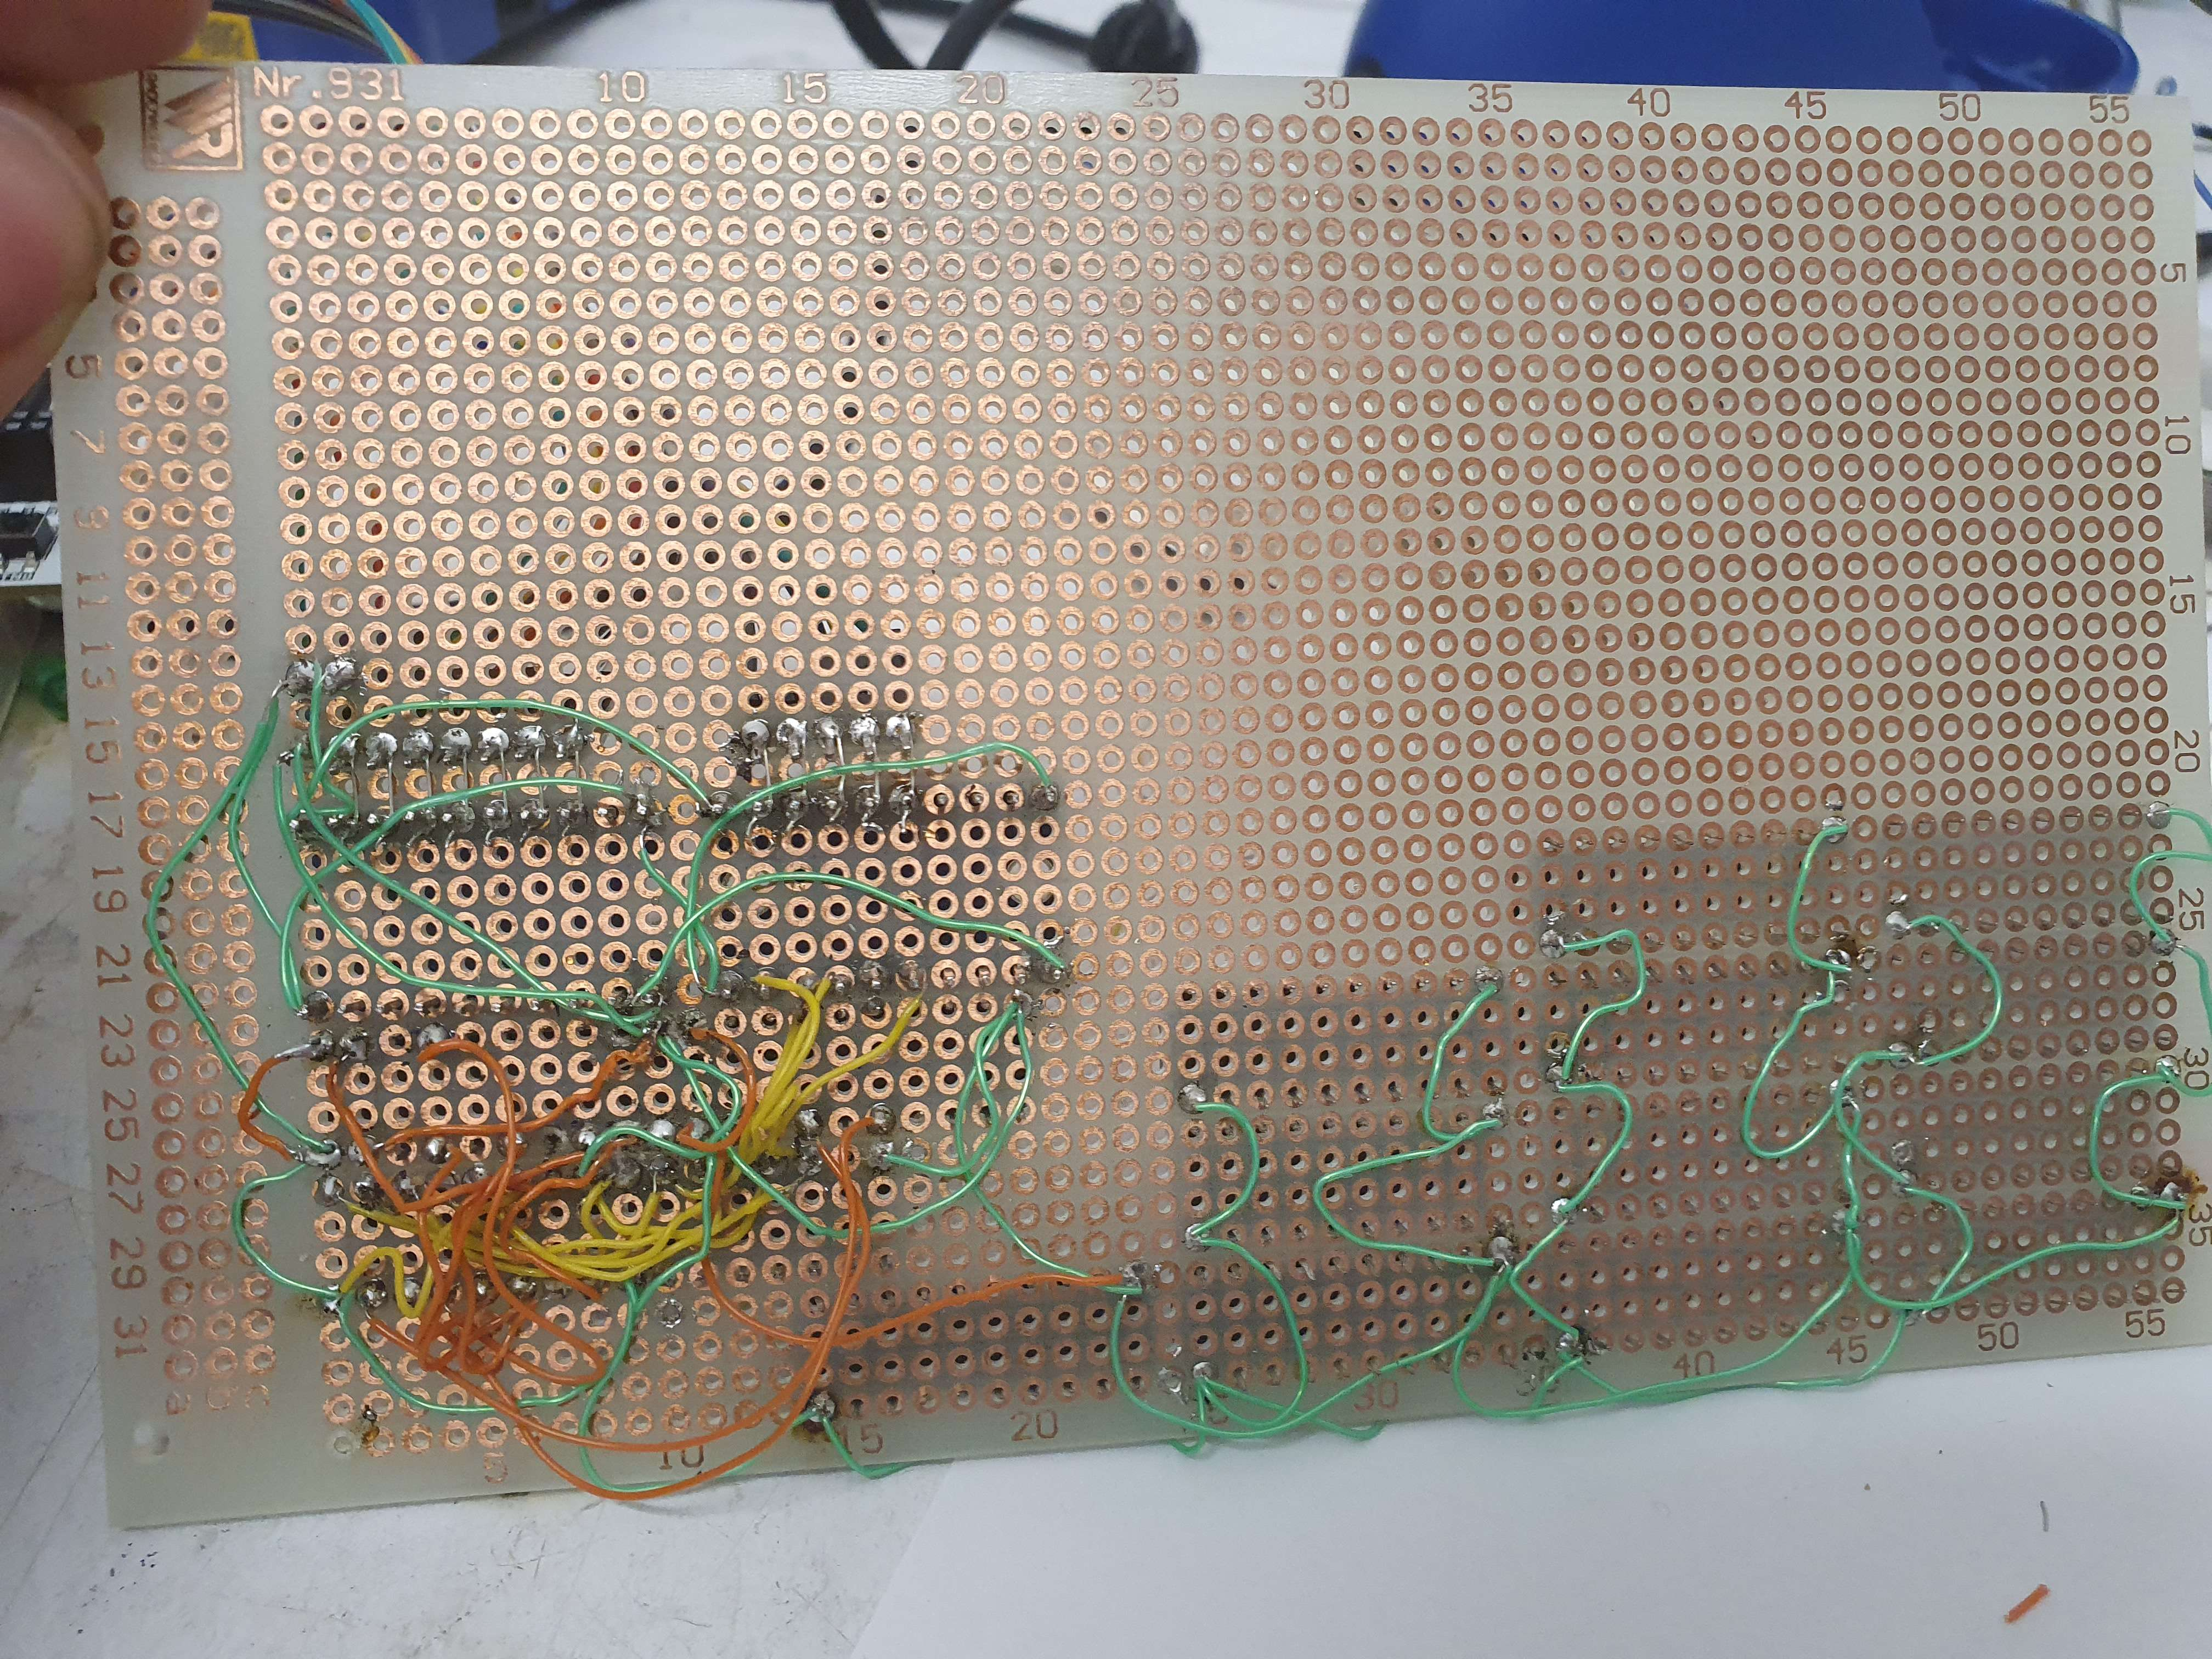
\includegraphics[scale=0.07]{pictures/Soudure proche.jpg}
    \end{center}
\end{frame}

\begin{frame}
    Nous sommes mauvais en soudure, et il y avait trop de court-circuit, donc nous avons abandonné.
    Finalement, nous avons utilisé une breadboard (pas besoin de soudures) et seulement 6 afficheurs,
    on peut changer de mode d'affichage avec les boutons. Nous pouvons afficher HH/MM/SS, YY/MO/DD
    ou YYYY/MO.
\end{frame}

\end{document}